\chapter{Ultrasound}
\label{ch:ultrasound}

% Chapter-opening illustrated modality infographic.
\begin{center}
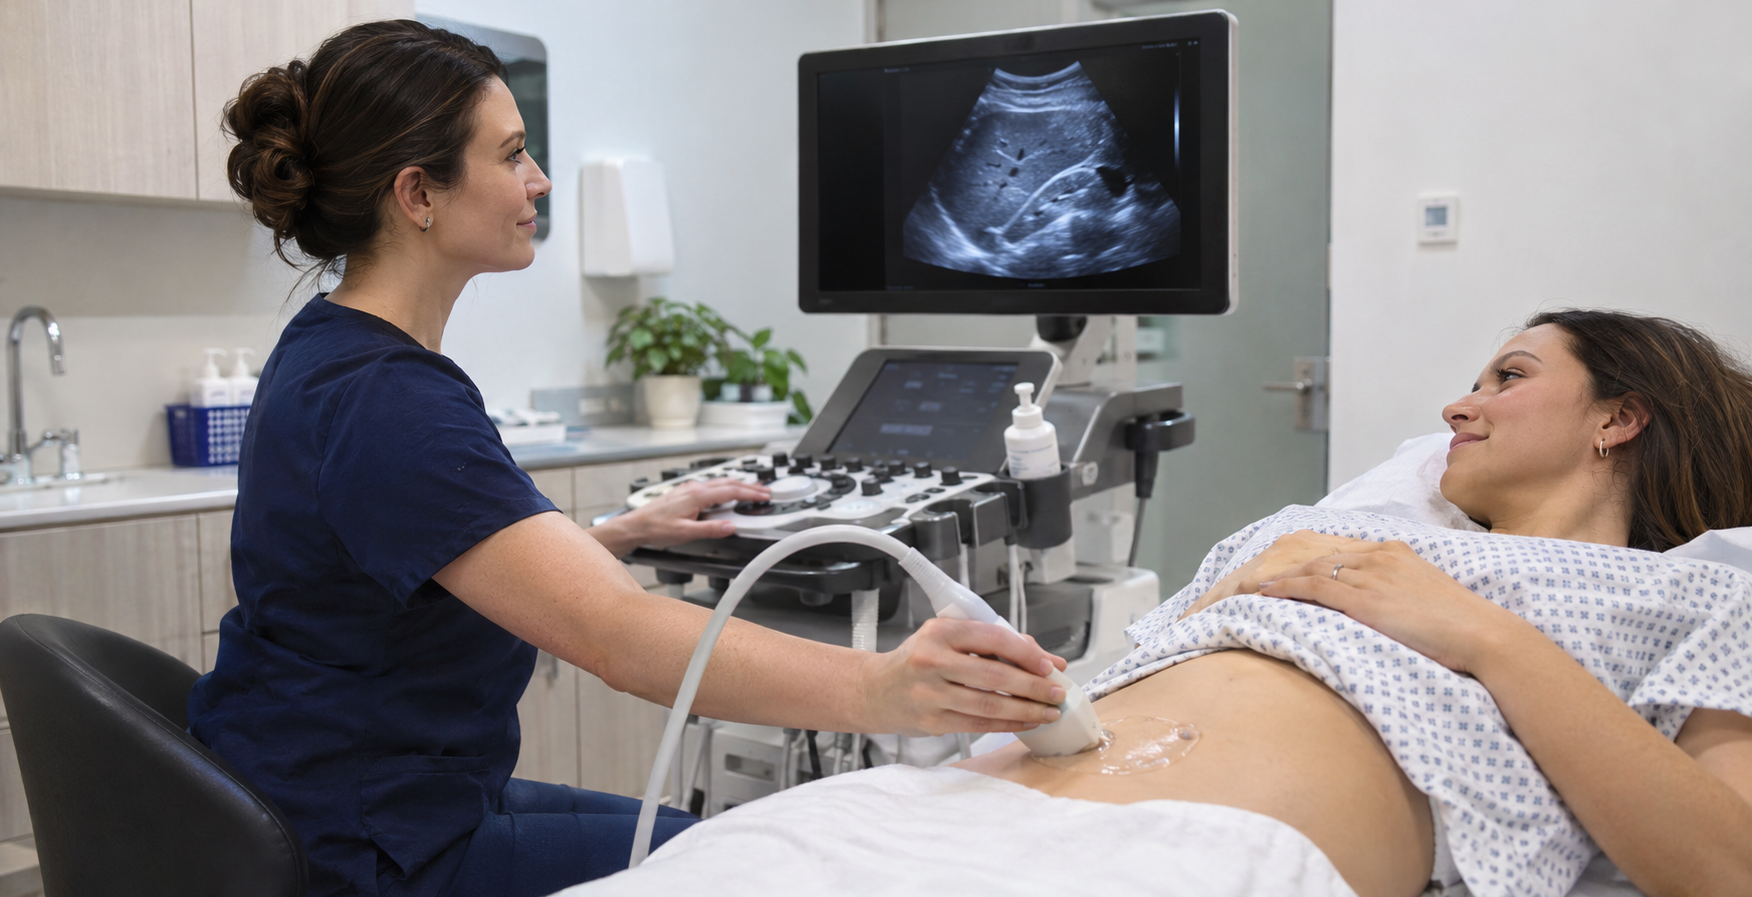
\includegraphics[width=\textwidth,keepaspectratio]{modalities/infographics/ultrasound_realistic.png}
\end{center}
\begin{center}\footnotesize Coupling gel removes air between the probe and skin so sound can enter the body; the returning echoes form a real-time image. Gas and bone can limit the acoustic window. AI-generated illustration; the ultrasound panel is not a clinical study.\end{center}

\section{Overview}
Diagnostic ultrasound (ultrasonography) uses high-frequency sound waves to visualize anatomical structures, blood flow, tissue abnormalities, and physiological movements in real time. Unlike conventional X-rays, ultrasound does not use ionizing radiation.

This catalogue covers diseases and conditions for which ultrasound has established clinical diagnostic utility. It includes conventional B-mode ultrasound, Doppler ultrasound, echocardiography, transvaginal ultrasound, and musculoskeletal ultrasound, while excluding purely therapeutic applications and procedural guidance.

The 263 entries form a preliminary catalogue of diseases, conditions, and observable abnormalities. They are not all independently diagnosable using ultrasound; some require alternative imaging, histopathology, or laboratory confirmation. Individual guideline validation is necessary before using this catalogue as diagnostic ground truth.

\section{Where ultrasound is used}
The following numbered entries present common diagnostic applications by anatomical system. Ultrasound may detect or characterize an abnormality without establishing its cause. A negative study does not exclude disease when sensitivity is limited. Findings should be interpreted with symptoms, examination, laboratory results, and other imaging.

\subsection{Liver}
\begin{enumerate}[leftmargin=*,itemsep=0.45em,topsep=0.4em]
\item \textbf{Budd--Chiari syndrome.} Useful imaging findings include: Hepatic venous obstruction.
\item \textbf{Congestive hepatopathy.} Useful imaging findings include: Dilated hepatic veins and inferior vena cava.
\item \textbf{Hepatic hemangioma.} Useful imaging findings include: Well-defined hyperechoic lesion.
\item \textbf{Hepatic metastases.} Useful imaging findings include: Multiple lesions may be detected, sometimes with a target appearance. Appearance alone cannot establish metastatic origin.
\item \textbf{Hepatic steatosis.} Useful imaging findings include: Increased hepatic echogenicity.
\item \textbf{Hepatocellular carcinoma.} Useful imaging findings include: Surveillance may detect a liver observation in an at-risk patient. A solid lesion is nonspecific and requires diagnostic characterization.
\item \textbf{Hepatomegaly.} Useful imaging findings include: Increased liver dimensions.
\item \textbf{Hydatid cyst.} Useful imaging findings include: Daughter cysts, detached membranes.
\item \textbf{Liver abscess.} Useful imaging findings include: Complex hypoechoic lesion with internal debris.
\item \textbf{Liver cirrhosis.} Useful imaging findings include: Nodular surface, coarse echotexture.
\item \textbf{Polycystic liver disease.} Useful imaging findings include: Multiple hepatic cysts.
\item \textbf{Portal hypertension.} Useful imaging findings include: Portosystemic collaterals, abnormal portal flow.
\item \textbf{Portal vein thrombosis.} Useful imaging findings include: Intraluminal thrombus, absent or reduced flow.
\item \textbf{Simple hepatic cyst.} Useful imaging findings include: Anechoic lesion with posterior acoustic enhancement.
\end{enumerate}

\subsection{Gallbladder and biliary system}
\begin{enumerate}[leftmargin=*,itemsep=0.45em,topsep=0.4em]
\item \textbf{Acalculous cholecystitis.} Useful imaging findings include: Inflammatory changes without gallstones.
\item \textbf{Acute cholecystitis.} Useful imaging findings include: Wall thickening, pericholecystic fluid, sonographic Murphy sign.
\item \textbf{Adenomyomatosis.} Useful imaging findings include: Comet-tail artifacts, intramural cystic spaces.
\item \textbf{Biliary obstruction.} Useful imaging findings include: Dilated bile ducts.
\item \textbf{Choledochal cyst.} Useful imaging findings include: Cystic bile duct dilatation.
\item \textbf{Choledocholithiasis.} Useful imaging findings include: Echogenic bile duct calculi.
\item \textbf{Cholelithiasis.} Useful imaging findings include: Echogenic calculi with posterior acoustic shadowing.
\item \textbf{Chronic cholecystitis.} Useful imaging findings include: Contracted gallbladder, wall thickening.
\item \textbf{Gallbladder carcinoma.} Useful imaging findings include: Irregular mass or asymmetric wall thickening.
\item \textbf{Gallbladder hydrops.} Useful imaging findings include: Markedly distended gallbladder.
\item \textbf{Gallbladder polyps.} Useful imaging findings include: Nonmobile mural projections.
\item \textbf{Gallbladder sludge.} Useful imaging findings include: Dependent low-level echoes.
\end{enumerate}

\subsection{Pancreas}
\begin{enumerate}[leftmargin=*,itemsep=0.45em,topsep=0.4em]
\item \textbf{Acute pancreatitis.} Useful imaging findings include: Enlarged hypoechoic pancreas.
\item \textbf{Chronic pancreatitis.} Useful imaging findings include: Heterogeneous echotexture, calcifications.
\item \textbf{Pancreatic calcification.} Useful imaging findings include: Echogenic foci with acoustic shadowing.
\item \textbf{Pancreatic carcinoma.} Useful imaging findings include: Irregular hypoechoic mass.
\item \textbf{Pancreatic cyst.} Useful imaging findings include: Anechoic or complex cystic lesion.
\item \textbf{Pancreatic duct dilatation.} Useful imaging findings include: Enlarged pancreatic duct.
\item \textbf{Pancreatic pseudocyst.} Useful imaging findings include: Encapsulated fluid collection.
\end{enumerate}

Transabdominal ultrasound has limitations in pancreatic imaging because of overlying bowel gas. CT, MRI, and endoscopic ultrasound are frequently preferred.

\subsection{Kidneys}
\begin{enumerate}[leftmargin=*,itemsep=0.45em,topsep=0.4em]
\item \textbf{Acute pyelonephritis.} Useful imaging findings include: Ultrasound may be normal or show nonspecific focal swelling or altered echogenicity. It is mainly used to assess obstruction or complications.
\item \textbf{Chronic kidney disease.} Useful imaging findings include: Increased cortical echogenicity, cortical thinning.
\item \textbf{Complex renal cyst.} Useful imaging findings include: Internal septations or solid components.
\item \textbf{Duplex collecting system.} Useful imaging findings include: Duplicated renal collecting structures.
\item \textbf{Ectopic kidney.} Useful imaging findings include: Abnormal renal location.
\item \textbf{Horseshoe kidney.} Useful imaging findings include: Fusion of renal poles.
\item \textbf{Hydronephrosis.} Useful imaging findings include: Dilated renal collecting system.
\item \textbf{Medullary nephrocalcinosis.} Useful imaging findings include: Echogenic renal pyramids.
\item \textbf{Multicystic dysplastic kidney.} Useful imaging findings include: Multiple noncommunicating cysts.
\item \textbf{Nephrolithiasis.} Useful imaging findings include: Echogenic calculus with acoustic shadowing.
\item \textbf{Polycystic kidney disease.} Useful imaging findings include: Multiple bilateral renal cysts.
\item \textbf{Renal abscess.} Useful imaging findings include: Complex fluid collection.
\item \textbf{Renal angiomyolipoma.} Useful imaging findings include: Typically hyperechoic renal mass.
\item \textbf{Renal artery stenosis.} Useful imaging findings include: Doppler may show increased velocity. Technical limitations can affect the study, and stenosis alone does not establish renovascular hypertension.
\item \textbf{Renal atrophy.} Useful imaging findings include: Reduced renal dimensions.
\item \textbf{Renal cell carcinoma.} Useful imaging findings include: Solid renal mass.
\item \textbf{Renal vein thrombosis.} Useful imaging findings include: Abnormal or absent venous flow may support thrombosis. Further imaging may be needed when the examination is limited or equivocal.
\item \textbf{Simple renal cyst.} Useful imaging findings include: Anechoic, thin-walled lesion.
\end{enumerate}

\subsection{Urinary bladder and prostate}
\begin{enumerate}[leftmargin=*,itemsep=0.45em,topsep=0.4em]
\item \textbf{Benign prostatic hyperplasia.} Useful imaging findings include: Increased prostate volume.
\item \textbf{Bladder diverticulum.} Useful imaging findings include: Outpouching of the bladder wall.
\item \textbf{Bladder outlet obstruction.} Useful imaging findings include: Increased postvoid residual, trabeculation.
\item \textbf{Bladder stones.} Useful imaging findings include: Mobile echogenic structures with shadowing.
\item \textbf{Bladder tumor.} Useful imaging findings include: Mural soft-tissue mass.
\item \textbf{Prostatic abscess.} Useful imaging findings include: Complex hypoechoic collection.
\item \textbf{Prostatic cyst.} Useful imaging findings include: Anechoic intraprostatic lesion.
\item \textbf{Ureterocele.} Useful imaging findings include: Cystic structure near the ureteric orifice.
\item \textbf{Urinary retention.} Useful imaging findings include: Distended urinary bladder.
\end{enumerate}

\subsection{Spleen}
\begin{enumerate}[leftmargin=*,itemsep=0.45em,topsep=0.4em]
\item \textbf{Splenic abscess.} Useful imaging findings include: Complex hypoechoic collection.
\item \textbf{Splenic cyst.} Useful imaging findings include: Anechoic lesion.
\item \textbf{Splenic hemangioma.} Useful imaging findings include: Focal lesion with variable echogenicity.
\item \textbf{Splenic hematoma.} Useful imaging findings include: Subcapsular or intraparenchymal collection.
\item \textbf{Splenic infarction.} Useful imaging findings include: Peripheral wedge-shaped hypoechoic region.
\item \textbf{Splenic rupture.} Useful imaging findings include: Parenchymal disruption, perisplenic fluid.
\item \textbf{Splenomegaly.} Useful imaging findings include: Increased splenic dimensions.
\end{enumerate}

\subsection{Gastrointestinal system}
\begin{enumerate}[leftmargin=*,itemsep=0.45em,topsep=0.4em]
\item \textbf{Acute appendicitis.} Useful imaging findings include: A dilated, noncompressible appendix supports the diagnosis when visualized. Nonvisualization does not exclude appendicitis.
\item \textbf{Crohn disease.} Useful imaging findings include: Bowel wall thickening, increased vascularity.
\item \textbf{Diverticulitis.} Useful imaging findings include: Inflamed diverticulum, surrounding echogenic fat.
\item \textbf{Hypertrophic pyloric stenosis.} Useful imaging findings include: Thickened and elongated pyloric muscle.
\item \textbf{Incisional hernia.} Useful imaging findings include: Herniation through a surgical defect.
\item \textbf{Inguinal hernia.} Useful imaging findings include: Protrusion of abdominal contents.
\item \textbf{Intussusception.} Useful imaging findings include: Target sign, pseudokidney sign.
\item \textbf{Mesenteric lymphadenitis.} Useful imaging findings include: Enlarged mesenteric lymph nodes.
\item \textbf{Midgut volvulus.} Useful imaging findings include: Whirlpool sign.
\item \textbf{Necrotizing enterocolitis.} Useful imaging findings include: Ultrasound may show bowel-wall pneumatosis, thinning, absent perfusion, or complex fluid. It supplements radiographs and clinical assessment.
\item \textbf{Small bowel obstruction.} Useful imaging findings include: Dilated fluid-filled bowel loops.
\item \textbf{Ulcerative colitis.} Useful imaging findings include: Colonic wall thickening.
\item \textbf{Umbilical hernia.} Useful imaging findings include: Herniation through an umbilical defect.
\end{enumerate}

\subsection{Female reproductive system}
\begin{enumerate}[leftmargin=*,itemsep=0.45em,topsep=0.4em]
\item \textbf{Adenomyosis.} Useful imaging findings include: Heterogeneous myometrium, myometrial cysts.
\item \textbf{Bicornuate uterus.} Useful imaging findings include: Two uterine horns and external fundal cleft.
\item \textbf{Cesarean scar defect.} Useful imaging findings include: Hypoechoic indentation at the uterine scar.
\item \textbf{Endometrial carcinoma.} Useful imaging findings include: Irregular endometrial thickening or mass.
\item \textbf{Endometrial hyperplasia.} Useful imaging findings include: Endometrial thickening.
\item \textbf{Endometrial polyp.} Useful imaging findings include: Focal endometrial lesion, feeding vessel.
\item \textbf{Hemorrhagic ovarian cyst.} Useful imaging findings include: Reticular internal echoes.
\item \textbf{Hydrosalpinx.} Useful imaging findings include: Elongated fluid-filled tubular structure.
\item \textbf{Ovarian carcinoma.} Useful imaging findings include: A complex mass with solid tissue or papillary projections is suspicious but cannot establish histology.
\item \textbf{Ovarian dermoid cyst.} Useful imaging findings include: Echogenic components, acoustic shadowing.
\item \textbf{Ovarian endometrioma.} Useful imaging findings include: Ground-glass internal echoes.
\item \textbf{Ovarian torsion.} Useful imaging findings include: An enlarged ovary or twisted pedicle supports torsion. Preserved Doppler flow does not exclude it.
\item \textbf{Pelvic endometriosis.} Useful imaging findings include: Expert ultrasound may detect some deep endometriotic lesions. A normal scan does not exclude superficial disease.
\item \textbf{Pelvic organ prolapse.} Useful imaging findings include: Dynamic descent of pelvic structures.
\item \textbf{Polycystic ovarian morphology.} Useful imaging findings include: Increased follicle number or ovarian volume may meet imaging criteria. This morphology alone does not diagnose polycystic ovary syndrome.
\item \textbf{Pyosalpinx.} Useful imaging findings include: Dilated tube with internal debris.
\item \textbf{Retained products of conception.} Useful imaging findings include: Intrauterine echogenic tissue, variable vascularity.
\item \textbf{Septate uterus.} Useful imaging findings include: Internal uterine septum.
\item \textbf{Simple ovarian cyst.} Useful imaging findings include: Thin-walled anechoic lesion.
\item \textbf{Tubo-ovarian abscess.} Useful imaging findings include: Complex inflammatory adnexal mass.
\item \textbf{Unicornuate uterus.} Useful imaging findings include: Asymmetric single uterine horn.
\item \textbf{Uterine fibroids.} Useful imaging findings include: Well-defined solid myometrial masses.
\end{enumerate}

\subsection{Obstetric and fetal conditions}
\begin{enumerate}[leftmargin=*,itemsep=0.45em,topsep=0.4em]
\item \textbf{Anembryonic pregnancy.} Useful imaging findings include: Empty gestational sac meeting diagnostic criteria.
\item \textbf{Anencephaly.} Useful imaging findings include: Absence of major cranial structures.
\item \textbf{Cervical insufficiency.} Useful imaging findings include: Shortened cervix, cervical funneling.
\item \textbf{Congenital diaphragmatic hernia.} Useful imaging findings include: Abdominal organs within the fetal thorax.
\item \textbf{Early pregnancy loss.} Useful imaging findings include: Absent embryonic cardiac activity meeting diagnostic criteria.
\item \textbf{Ectopic pregnancy.} Useful imaging findings include: Extrauterine gestational sac or adnexal mass.
\item \textbf{Fetal congenital heart defects.} Useful imaging findings include: Targeted fetal echocardiography can identify many structural defects. Routine screening does not detect every defect.
\item \textbf{Fetal growth restriction.} Useful imaging findings include: Estimated fetal weight or abdominal circumference is interpreted by gestational-age percentiles and clinical context. A single small measurement alone may not establish pathologic growth restriction.
\item \textbf{Fetal hydrocephalus.} Useful imaging findings include: Ventricular dilatation.
\item \textbf{Fetal hydronephrosis.} Useful imaging findings include: Dilated renal collecting system.
\item \textbf{Fetal hydrops.} Useful imaging findings include: Abnormal fluid in multiple fetal compartments.
\item \textbf{Fetal macrosomia.} Useful imaging findings include: Increased estimated fetal weight.
\item \textbf{Fetal renal agenesis.} Useful imaging findings include: Absent renal structures.
\item \textbf{Fetal skeletal dysplasia.} Useful imaging findings include: Disproportionate measurements or abnormal bone morphology may raise suspicion. Some dysplasias are not detectable on routine ultrasound.
\item \textbf{Gastroschisis.} Useful imaging findings include: Externalized bowel without a covering membrane.
\item \textbf{Hydatidiform mole.} Useful imaging findings include: Multicystic intrauterine tissue.
\item \textbf{Oligohydramnios.} Useful imaging findings include: Reduced amniotic fluid volume.
\item \textbf{Omphalocele.} Useful imaging findings include: Membrane-covered abdominal wall defect.
\item \textbf{Placenta accreta spectrum.} Useful imaging findings include: Placental lacunae, abnormal vascularity.
\item \textbf{Placenta previa.} Useful imaging findings include: Placenta covering the internal cervical os.
\item \textbf{Placental abruption.} Useful imaging findings include: A retroplacental hematoma may be visible. A normal ultrasound does not exclude abruption.
\item \textbf{Polyhydramnios.} Useful imaging findings include: Increased amniotic fluid volume.
\item \textbf{Spina bifida.} Useful imaging findings include: Spinal defect, associated cranial signs.
\item \textbf{Twin-to-twin transfusion syndrome.} Useful imaging findings include: Discordant amniotic fluid volumes.
\item \textbf{Vasa previa.} Useful imaging findings include: Fetal vessels crossing the internal cervical os.
\end{enumerate}

\subsection{Breast}
\begin{enumerate}[leftmargin=*,itemsep=0.45em,topsep=0.4em]
\item \textbf{Breast abscess.} Useful imaging findings include: Complex fluid collection.
\item \textbf{Breast carcinoma.} Useful imaging findings include: An irregular nonparallel mass may be suspicious. Ultrasound appearance cannot establish histology, which requires biopsy.
\item \textbf{Breast hematoma.} Useful imaging findings include: Complex fluid collection.
\item \textbf{Complicated breast cyst.} Useful imaging findings include: Internal low-level echoes.
\item \textbf{Duct ectasia.} Useful imaging findings include: Dilated mammary ducts.
\item \textbf{Fat necrosis.} Useful imaging findings include: Variable cystic or solid appearance.
\item \textbf{Fibroadenoma.} Useful imaging findings include: Oval, circumscribed hypoechoic mass.
\item \textbf{Galactocele.} Useful imaging findings include: Variable echogenicity, sometimes fat-fluid level.
\item \textbf{Intraductal papilloma.} Useful imaging findings include: Solid intraductal mass.
\item \textbf{Mastitis.} Useful imaging findings include: Increased vascularity and tissue edema.
\item \textbf{Phyllodes tumor.} Useful imaging findings include: A large heterogeneous mass may raise suspicion, but imaging cannot reliably distinguish phyllodes tumor from fibroadenoma or establish its grade.
\item \textbf{Postoperative seroma.} Useful imaging findings include: Fluid collection.
\item \textbf{Silicone implant rupture.} Useful imaging findings include: A stepladder sign can indicate intracapsular rupture and a snowstorm appearance can indicate extracapsular silicone. Equivocal examinations may require MRI.
\item \textbf{Simple breast cyst.} Useful imaging findings include: Anechoic lesion with posterior enhancement.
\end{enumerate}

\subsection{Thyroid and parathyroid glands}
\begin{enumerate}[leftmargin=*,itemsep=0.45em,topsep=0.4em]
\item \textbf{Follicular thyroid neoplasm.} Useful imaging findings include: Ultrasound can characterize a solid nodule but cannot distinguish follicular adenoma from carcinoma. Histology assessing capsular or vascular invasion is required.
\item \textbf{Graves disease.} Useful imaging findings include: Diffuse hypervascularity.
\item \textbf{Hashimoto thyroiditis.} Useful imaging findings include: Heterogeneous hypoechoic gland.
\item \textbf{Multinodular goiter.} Useful imaging findings include: Multiple thyroid nodules.
\item \textbf{Papillary thyroid carcinoma.} Useful imaging findings include: Suspicious hypoechoic nodule, punctate echogenic foci.
\item \textbf{Parathyroid adenoma.} Useful imaging findings include: A hypoechoic lesion can help localize a suspected abnormal gland. Ultrasound does not establish biochemical hyperparathyroidism.
\item \textbf{Subacute thyroiditis.} Useful imaging findings include: Patchy hypoechoic regions.
\item \textbf{Thyroid abscess.} Useful imaging findings include: Complex fluid collection.
\item \textbf{Thyroid cyst.} Useful imaging findings include: Anechoic or complex cystic lesion.
\item \textbf{Thyroid nodule.} Useful imaging findings include: Focal solid, cystic, or mixed lesion.
\end{enumerate}

\subsection{Cardiovascular system: echocardiography}
\begin{enumerate}[leftmargin=*,itemsep=0.45em,topsep=0.4em]
\item \textbf{Aortic regurgitation.} Useful imaging findings include: Retrograde diastolic blood flow.
\item \textbf{Aortic stenosis.} Useful imaging findings include: Restricted valve opening, increased flow velocity.
\item \textbf{Atrial myxoma.} Useful imaging findings include: Mobile intracardiac mass.
\item \textbf{Atrial septal defect.} Useful imaging findings include: Interatrial communication.
\item \textbf{Cardiac tamponade.} Useful imaging findings include: Chamber collapse, abnormal respiratory flow variation.
\item \textbf{Constrictive pericarditis.} Useful imaging findings include: Abnormal septal motion, ventricular interdependence.
\item \textbf{Dilated cardiomyopathy.} Useful imaging findings include: Dilated ventricles, reduced contractility.
\item \textbf{Heart failure with preserved ejection fraction.} Useful imaging findings include: Echocardiographic structure and diastolic indices support assessment. Filling pressure estimates are imperfect and must be interpreted with clinical findings.
\item \textbf{Heart failure with reduced ejection fraction.} Useful imaging findings include: Reduced left ventricular ejection fraction.
\item \textbf{Hypertrophic cardiomyopathy.} Useful imaging findings include: Abnormal myocardial thickening.
\item \textbf{Infective endocarditis.} Useful imaging findings include: Echocardiography may show vegetations or complications. A negative transthoracic study does not exclude endocarditis when suspicion remains high. Transesophageal echocardiography may be needed.
\item \textbf{Left ventricular thrombus.} Useful imaging findings include: Intracavitary mass.
\item \textbf{Mitral regurgitation.} Useful imaging findings include: Retrograde systolic blood flow.
\item \textbf{Mitral stenosis.} Useful imaging findings include: Restricted mitral valve opening.
\item \textbf{Mitral valve prolapse.} Useful imaging findings include: Systolic leaflet displacement.
\item \textbf{Patent ductus arteriosus.} Useful imaging findings include: Persistent abnormal vascular connection.
\item \textbf{Pericardial effusion.} Useful imaging findings include: Fluid surrounding the heart.
\item \textbf{Pulmonary hypertension.} Useful imaging findings include: Echocardiography estimates the probability and pressure. Right-heart catheterization confirms the hemodynamic diagnosis.
\item \textbf{Pulmonary valve stenosis.} Useful imaging findings include: Increased transvalvular flow velocity.
\item \textbf{Regional myocardial dysfunction.} Useful imaging findings include: Regional wall-motion abnormalities.
\item \textbf{Restrictive cardiomyopathy.} Useful imaging findings include: Abnormal ventricular filling.
\item \textbf{Tetralogy of Fallot.} Useful imaging findings include: Characteristic congenital cardiac abnormalities.
\item \textbf{Tricuspid regurgitation.} Useful imaging findings include: Retrograde flow across the tricuspid valve.
\item \textbf{Ventricular aneurysm.} Useful imaging findings include: Abnormal ventricular outpouching.
\item \textbf{Ventricular septal defect.} Useful imaging findings include: Interventricular communication.
\end{enumerate}

\subsection{Vascular system: Doppler ultrasound}
\begin{enumerate}[leftmargin=*,itemsep=0.45em,topsep=0.4em]
\item \textbf{Abdominal aortic aneurysm.} Useful imaging findings include: Increased aortic diameter.
\item \textbf{Acute arterial occlusion.} Useful imaging findings include: Absent arterial flow.
\item \textbf{Arterial pseudoaneurysm.} Useful imaging findings include: To-and-fro flow at the neck.
\item \textbf{Arteriovenous fistula.} Useful imaging findings include: High-velocity turbulent flow.
\item \textbf{Arteriovenous malformation.} Useful imaging findings include: Abnormal vascular channels.
\item \textbf{Carotid artery stenosis.} Useful imaging findings include: Doppler velocity and plaque support stenosis grading. Confirmatory imaging may be needed for intervention planning.
\item \textbf{Chronic venous insufficiency.} Useful imaging findings include: Abnormal venous reflux.
\item \textbf{Deep vein thrombosis.} Useful imaging findings include: Noncompressible vein.
\item \textbf{Peripheral arterial aneurysm.} Useful imaging findings include: Focal arterial dilatation.
\item \textbf{Peripheral arterial disease.} Useful imaging findings include: Abnormal waveforms suggest disease. Duplex assessment and ankle-brachial index help determine its location and hemodynamic significance.
\item \textbf{Subclavian steal syndrome.} Useful imaging findings include: Reversed vertebral arterial flow.
\item \textbf{Superficial venous thrombosis.} Useful imaging findings include: Intraluminal venous thrombus.
\item \textbf{Varicose veins.} Useful imaging findings include: Dilated tortuous superficial veins.
\end{enumerate}

\subsection{Musculoskeletal system}
\begin{enumerate}[leftmargin=*,itemsep=0.45em,topsep=0.4em]
\item \textbf{Achilles tendon rupture.} Useful imaging findings include: Disrupted tendon fibers.
\item \textbf{Baker cyst.} Useful imaging findings include: Popliteal fluid collection.
\item \textbf{Bursitis.} Useful imaging findings include: Fluid-filled distended bursa.
\item \textbf{Calcific tendinitis.} Useful imaging findings include: Echogenic intratendinous deposits.
\item \textbf{Carpal tunnel syndrome.} Useful imaging findings include: Enlarged median nerve.
\item \textbf{CPPD disease.} Useful imaging findings include: Cartilage deposits may be seen. The appearance is operator-dependent and does not replace crystal analysis when confirmation is needed.
\item \textbf{Developmental dysplasia of the hip.} Useful imaging findings include: Abnormal femoral head coverage.
\item \textbf{Enthesitis.} Useful imaging findings include: Tendon insertion abnormalities.
\item \textbf{Ganglion cyst.} Useful imaging findings include: Cystic periarticular lesion.
\item \textbf{Gout.} Useful imaging findings include: The double-contour sign or tophi can support gout. Absence of these findings does not exclude early disease, and other crystal disease can overlap.
\item \textbf{Joint effusion.} Useful imaging findings include: Intra-articular fluid.
\item \textbf{Morton neuroma.} Useful imaging findings include: Hypoechoic interdigital mass.
\item \textbf{Muscle hematoma.} Useful imaging findings include: Intramuscular collection.
\item \textbf{Muscle tear.} Useful imaging findings include: Disrupted muscle architecture.
\item \textbf{Plantar fasciitis.} Useful imaging findings include: Thickened plantar fascia.
\item \textbf{Rheumatoid arthritis.} Useful imaging findings include: Ultrasound can show synovitis, Doppler activity, and erosions. These findings are not specific and do not replace clinical classification.
\item \textbf{Rotator cuff tear.} Useful imaging findings include: Tendon discontinuity.
\item \textbf{Synovitis.} Useful imaging findings include: Synovial thickening and hypervascularity.
\item \textbf{Tendinopathy.} Useful imaging findings include: Tendon thickening and altered echogenicity.
\item \textbf{Tenosynovitis.} Useful imaging findings include: Tendon sheath fluid and inflammation.
\item \textbf{Trigger finger.} Useful imaging findings include: Thickening of the A1 pulley.
\item \textbf{Ulnar nerve entrapment.} Useful imaging findings include: Enlarged or dynamically displaced ulnar nerve.
\end{enumerate}

\subsection{Male reproductive system}
\begin{enumerate}[leftmargin=*,itemsep=0.45em,topsep=0.4em]
\item \textbf{Epididymitis.} Useful imaging findings include: Enlarged hypervascular epididymis.
\item \textbf{Hematocele.} Useful imaging findings include: Complex fluid surrounding the testicle.
\item \textbf{Hydrocele.} Useful imaging findings include: Fluid surrounding the testicle.
\item \textbf{Orchitis.} Useful imaging findings include: Increased testicular vascularity.
\item \textbf{Spermatocele.} Useful imaging findings include: Cystic epididymal lesion.
\item \textbf{Testicular abscess.} Useful imaging findings include: Complex intratesticular collection.
\item \textbf{Testicular carcinoma.} Useful imaging findings include: Solid intratesticular mass.
\item \textbf{Testicular microlithiasis.} Useful imaging findings include: Multiple punctate echogenic foci.
\item \textbf{Testicular rupture.} Useful imaging findings include: Disruption of the tunica albuginea.
\item \textbf{Testicular torsion.} Useful imaging findings include: A twisted spermatic cord or reduced flow supports torsion. Preserved flow can occur and does not exclude torsion.
\item \textbf{Undescended testicle.} Useful imaging findings include: Testicle outside its normal scrotal location.
\item \textbf{Varicocele.} Useful imaging findings include: Dilated veins with reflux.
\end{enumerate}

\subsection{Ophthalmology}
\begin{enumerate}[leftmargin=*,itemsep=0.45em,topsep=0.4em]
\item \textbf{Choroidal detachment.} Useful imaging findings include: Dome-shaped elevated choroidal membranes.
\item \textbf{Choroidal melanoma.} Useful imaging findings include: Solid intraocular mass.
\item \textbf{Dislocated crystalline lens.} Useful imaging findings include: Abnormal lens position.
\item \textbf{Intraocular foreign body.} Useful imaging findings include: Echogenic foreign object.
\item \textbf{Optic disc drusen.} Useful imaging findings include: Highly reflective calcified deposits.
\item \textbf{Posterior scleritis.} Useful imaging findings include: A T-sign may be visible on B-scan ultrasound. Ophthalmic examination and other imaging may be needed.
\item \textbf{Posterior vitreous detachment.} Useful imaging findings include: Mobile detached vitreous membrane.
\item \textbf{Retinal detachment.} Useful imaging findings include: Elevated retinal membrane.
\item \textbf{Retinoblastoma.} Useful imaging findings include: Intraocular mass with possible calcifications.
\item \textbf{Vitreous hemorrhage.} Useful imaging findings include: Mobile internal vitreous echoes.
\end{enumerate}

\subsection{Pulmonary and thoracic ultrasound}
\begin{enumerate}[leftmargin=*,itemsep=0.45em,topsep=0.4em]
\item \textbf{Atelectasis.} Useful imaging findings include: Tissue-like lung appearance.
\item \textbf{Diaphragmatic paralysis.} Useful imaging findings include: Absent or paradoxical diaphragmatic movement.
\item \textbf{Empyema.} Useful imaging findings include: Complex or septated pleural fluid.
\item \textbf{Peripheral pneumonia.} Useful imaging findings include: Subpleural consolidation, air bronchograms.
\item \textbf{Peripheral pulmonary infarction.} Useful imaging findings include: A pleural-based wedge-shaped lesion may be visible but is nonspecific. Ultrasound cannot exclude pulmonary embolism or confirm infarction alone.
\item \textbf{Pleural effusion.} Useful imaging findings include: Fluid within the pleural space.
\item \textbf{Pneumothorax.} Useful imaging findings include: Absent lung sliding, lung point when visible.
\item \textbf{Pulmonary edema.} Useful imaging findings include: Multiple bilateral B-lines.
\end{enumerate}

\subsection{Superficial soft tissues and lymph nodes}
\begin{enumerate}[leftmargin=*,itemsep=0.45em,topsep=0.4em]
\item \textbf{Cellulitis.} Useful imaging findings include: Cobblestone appearance.
\item \textbf{Epidermoid cyst.} Useful imaging findings include: Circumscribed lesion with internal echoes.
\item \textbf{Lipoma.} Useful imaging findings include: Usually well-defined soft-tissue mass.
\item \textbf{Lymphedema.} Useful imaging findings include: Subcutaneous edema.
\item \textbf{Lymphoma.} Useful imaging findings include: Enlarged hypoechoic lymph nodes.
\item \textbf{Metastatic lymphadenopathy.} Useful imaging findings include: Abnormal nodal morphology.
\item \textbf{Pilomatricoma.} Useful imaging findings include: Superficial mass with calcifications.
\item \textbf{Reactive lymphadenopathy.} Useful imaging findings include: Enlarged nodes with preserved fatty hilum.
\item \textbf{Soft-tissue abscess.} Useful imaging findings include: Complex fluid collection.
\item \textbf{Soft-tissue foreign body.} Useful imaging findings include: Echogenic object with surrounding inflammation.
\end{enumerate}

\subsection{Neonatal cranial ultrasound}
\begin{enumerate}[leftmargin=*,itemsep=0.45em,topsep=0.4em]
\item \textbf{Agenesis of the corpus callosum.} Useful imaging findings include: Abnormal midline anatomy.
\item \textbf{Dandy--Walker malformation.} Useful imaging findings include: Abnormal posterior fossa structures.
\item \textbf{Germinal matrix hemorrhage.} Useful imaging findings include: Echogenic focus at the caudothalamic groove.
\item \textbf{Hydrocephalus.} Useful imaging findings include: Ventricular enlargement.
\item \textbf{Intraventricular hemorrhage.} Useful imaging findings include: Echogenic intraventricular blood.
\item \textbf{Periventricular leukomalacia.} Useful imaging findings include: Periventricular echogenicity or cystic changes.
\item \textbf{Porencephalic cyst.} Useful imaging findings include: Intracerebral cystic cavity.
\end{enumerate}

\subsection{Emergency abdominal ultrasound}
\begin{enumerate}[leftmargin=*,itemsep=0.45em,topsep=0.4em]
\item \textbf{Abdominal abscess.} Useful imaging findings include: Complex fluid collection.
\item \textbf{Abdominal hematoma.} Useful imaging findings include: Collection with variable echogenicity.
\item \textbf{Ascites.} Useful imaging findings include: Free intraperitoneal fluid.
\item \textbf{Hemoperitoneum.} Useful imaging findings include: Free intraperitoneal fluid in a trauma setting.
\item \textbf{Retroperitoneal mass.} Useful imaging findings include: Abnormal retroperitoneal lesion.
\end{enumerate}

\subsection{Summary}
\begin{center}
\begin{tabular}{@{}lr@{}}
\toprule
\textbf{Anatomical system} & \textbf{Conditions} \\
\midrule
Breast & 14 \\
Echocardiography & 25 \\
Emergency abdominal ultrasound & 5 \\
Female reproductive system & 22 \\
Gallbladder and biliary system & 12 \\
Gastrointestinal system & 13 \\
Kidneys & 18 \\
Liver & 14 \\
Male reproductive system & 12 \\
Musculoskeletal system & 22 \\
Neonatal cranial ultrasound & 7 \\
Obstetrics and fetal medicine & 25 \\
Ophthalmology & 10 \\
Pancreas & 7 \\
Pulmonary and thoracic system & 8 \\
Spleen & 7 \\
Superficial soft tissues & 10 \\
Thyroid and parathyroid glands & 10 \\
\textbf{Total} & \textbf{263} \\
Urinary bladder and prostate & 9 \\
\midrule
Vascular system & 13 \\
\bottomrule
\end{tabular}
\end{center}

\subsection{Authoritative sources for published ultrasound images}
\begin{longtable}{@{}p{0.40\textwidth}p{0.54\textwidth}@{}}
\toprule
\textbf{Source} & \textbf{Primary utility} \\
\midrule
\endfirsthead
\toprule
\textbf{Source} & \textbf{Primary utility} \\
\midrule
\endhead
ACR Appropriateness Criteria & Clinical indications for diagnostic imaging \\
American Institute of Ultrasound in Medicine & Ultrasound practice parameters \\
American Society of Echocardiography & Cardiac ultrasound \\
International Society of Ultrasound in Obstetrics and Gynecology & Obstetric and gynecological ultrasound \\
PubMed Central & Published clinical sonograms \\
Radiopaedia & Annotated diagnostic imaging cases \\
The Radiology Assistant & Radiological interpretation \\
UltrasoundCases.info & Clinical ultrasound pathology atlas \\
\bottomrule
\end{longtable}

\subsection{Acquisition techniques for dataset development}
For medical imaging dataset development, ultrasound images should additionally be classified by acquisition technique:
\begin{itemize}
    \item B-mode ultrasound
    \item M-mode ultrasound
    \item Color Doppler
    \item Power Doppler
    \item Spectral Doppler
    \item Contrast-enhanced ultrasound
    \item Ultrasound elastography
    \item 3D ultrasound
    \item 4D ultrasound
\end{itemize}

Ultrasound is used in the medical assessment of every condition listed here, but its role varies. Some entries name a sonographic finding rather than a disease that can be diagnosed from the image alone. A normal or technically limited examination may not exclude disease. Suspicious masses, suspected vascular disease, and clinically important negative examinations may require additional imaging, laboratory tests, pathology, or specialist assessment.

\subsection{Selected clinical guidance}
\begin{itemize}
    \item Society of Maternal-Fetal Medicine. \href{https://publications.smfm.org/publications/289-society-for-maternal-fetal-medicine-consult-series-52/}{Diagnosis and management of fetal growth restriction}.
    \item American College of Obstetricians and Gynecologists. \href{https://www.acog.org/clinical/clinical-guidance/committee-opinion/articles/2019/08/adnexal-torsion-in-adolescents}{Adnexal torsion in adolescents}.
    \item European Society of Cardiology. \href{https://academic.oup.com/eurheartj/article/44/39/3948/7243107}{Guidelines for the management of endocarditis}.
    \item American College of Radiology. \href{https://acsearch.acr.org/docs/3100728/Narrative/}{Appropriateness Criteria for breast implant evaluation}.
    \item American Society of Echocardiography. \href{https://www.asecho.org/wp-content/uploads/2025/07/Left-Ventricular-Diastolic-Function.pdf}{Recommendations for evaluation of left ventricular diastolic function and HFpEF}.
\end{itemize}
